
%%% SAMPLE_IJAM file
%%% For LaTeX users:


\documentclass[12pt]{article}
\usepackage{amsmath, amsthm}

\textwidth 12cm \textheight 18cm

%%% Theorem Like Envirouments

\newtheoremstyle{theorem}%name
{10pt} % space above
{10pt} % space below
{\sl} % bofy font
{\parindent} % indent - empty=no indent, \parindent= paragraph indent
{\bf} % thm head font
{. } % punctuation after thm head
{ } % space after thm head: `` ``=normal \newline=linebreak
{} % thm head specification
\theoremstyle{theorem}
\newtheorem{theorem}{Theorem}
\newtheorem{corollary}[theorem]{Corollary}

\newtheoremstyle{defi}%name
{10pt} % space above
{10pt} % space below
{\rm} % bofy font
{\parindent} % ident - empty=no indent, \parindent= paragraph indent
{\bf} % thm head font
{. } % punctuation after thm head
{ } % space after thm head: `` ``=normal \newline=linebreak
{} % thm head specification
\theoremstyle{defi}
\newtheorem{definition}[theorem]{Definition}

\def\proofname{\indent {\sl Proof.}}

%%%% Author's Definitions start here
\usepackage{graphicx}
%%%% End of Author's Definitions

\begin{document} %%%%%%%%%%%%%%%%%%%%%%%%%%

\title{The Wiener Polarity Index of Nanostar Dendrimers}

\author{Mohammad Farahani $^1$ , Mehdi  Alaeiyan $^1$, M. Ali Rostami $^2$\\[6pt], 
$^1$ Department of Mathematics\\ Iran University of Science and Technology (IUST)\\ Narmak, Tehran 16844, Iran
e-mail: ...,alaeiyan@iust.ac.ir\\[6pt]
$^2$ Department of Mathematics and Computer Science\\ Friedrich Schiller University Jena\\
Ernst-Abbe-Platz 2, Germany \\ e-mail: a.rostami@uni-jena.de
address}


\maketitle

\begin{abstract}

The Wiener polarity index of a graph $G$, denoted by $W_p (G)$, is defined as the number of unordered pairs of vertices that are at distance $3$ in $G$. As one of the classic topological indices, properties of $W_p (G)$ have been extensively studied for various graphs in the recent yearsIn this note an exact formula for the Wiener polarity index of nanostar dendrimers was computed.

\medskip

{\bf Math. Subject Classification:} ...

{\bf wiener polarity index, nanostar dendrimers, topological index} ...

\end{abstract}

%%%%%%%% Section 1 %%%%%%%%%%%%%%%%%%%%
\section{Introduction}
Molecular descriptors are playing significant role in chemistry, pharmacology, etc. Among them, topological indices have a prominent place \cite{1}. There are numerous of topological descriptors that have found some applications in theoretical chemistry, especially in QSPR/QSAR research. 

The so-called topological indices have received much attention in recent years, as they provide a strong correlation between a chemical compound's molecular structure and its properties. Some examples include, but not limited to Randic index \cite{2}, degree distance \cite{3}, connective eccentricity index \cite{4}, \cite{5}, Kirchho index \cite{6} , \cite{7}, and Balaban index \cite{8}. One of the oldest and well-studied such indices is the Wiener Index, defined as the sum of distances over all unordered vertex pairs in a graph $G$ \cite{9} and denoted by 
$$W(G) = \sum_{\{u,b\}\subseteq V(G)} d_G (u,v)$$,
where $d_G (u,v)$ (or simply $d (u,v)$ ) is the distance between $u$ and $v$ in $G$.

Throughout the years the Wiener index has been extensively studied and has become one of the best known (if not the best known) topological indices. In the same paper, another topological index was also introduced by Wiener, called the Wiener polarity index $W_p(G)$, which is defined as the number of unordered pairs of vertices that are at distance $3$ in $G$:
$$
W_p(G) = |\{\{u,b\}\subseteq V(G)| d(u,v) = 3\}|
$$

 Like the Wiener index, the Wiener polarity index has attracted much attention in recent years. By using the Wiener polarity index, Lukovits and Linert demonstrated quantitative structure-property relationships in a series of acyclic and cycle-containing hydrocarbons in \cite{10}. Hosoya~\cite{11} found a physical-chemical interpretation of $W_p(G)$. 

Du et al. \cite{12} described a linear time algorithm for computing the Wiener polarity index of trees and characterized the trees maximizing the index among all the trees of the given order. Later, Deng, Xiao and Tang characterized the extremal trees with respect to this index among all trees of order n and diameter $k$ \cite{13}. While for cycle-containing graphs, the maximum Wiener polarity index of unicyclic graphs and the corresponding extremal graphs were determined in \cite{14}. In \cite{15} Ma et al. determined the sharp upper bound of the Wiener polarity index among all bicyclic networks based on some graph transformations. Moreover, the extremal values of catacondensed hexagonal systems, hexagonal cacti and polyphenylene chains with respect to the Wiener polarity index were computed in \cite{16}. It was proved that the Wiener polarity index of fullerenes with $n$ carbon atoms is $(9n-60)/2$ in the same paper. Also in \cite{17}, the property of the Wiener polarity index in trees was investigated.
  
Dendrimers are highly branched macromolecules. They are being investigated for possible uses in nanotechnology, gene therapy, and other fields. Each dendrimer consists of a multifunctional core molecule with a dendritic wedge attached to each functional site. The core molecule without surrounding dendrons is usually referred to as zeros generation. Each successive repeat unit along all branches forms the next generation, 1st generation and 2nd generation and so on until the terminating generation. The topological study of these macromolecules is the aim of this article, see \cite{18}, \cite{19} and \cite{20}  for details. 
   In this paper an exact formulas for the Wiener polarity index of nanostar dendrimers was computed.
%%%%%%%% Section 2 %%%%%%%%%%%%%%%%%%%%
\section{Results and Discussions}

 A type of nanostar dendrimers is N-branched phenylacetylenes and it is shown by $NSB(n)$, some topological indices were obtained in \cite{21} , \cite{22} and \cite{23}. In Fig. \ref{fig1}, the molecular graph of $NSB(n)$ is shown. 
\begin{figure}
\label{fig1}
\centering
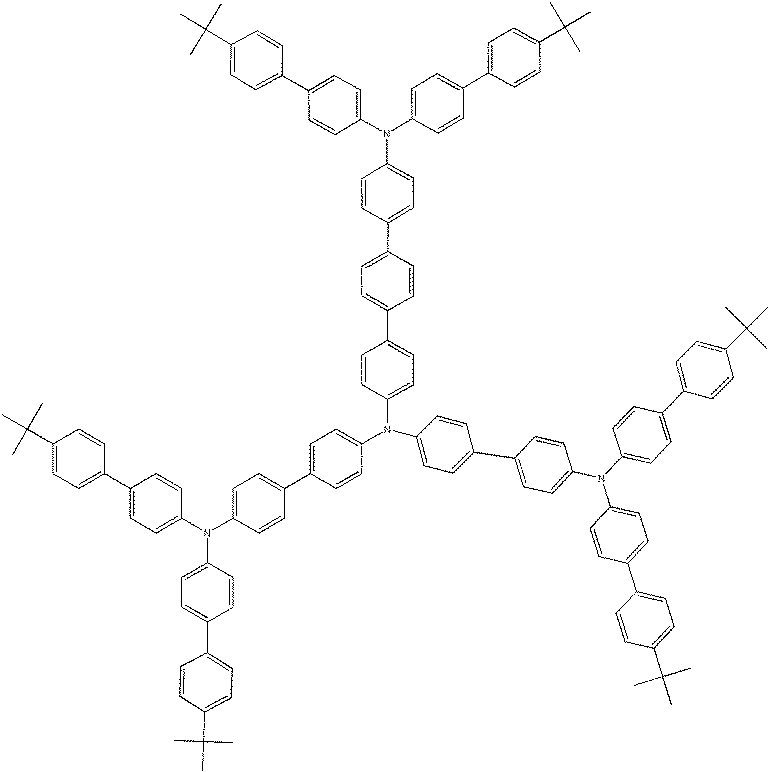
\includegraphics[width=0.7\linewidth]{img1}
\caption{The molecular graph of $NSB(n)$}
\end{figure}

In the following theorem we compute the Wiener polarity index of $NSB(n)$ for any integer $n\geq 1$.
\begin{theorem}
The Wiener polarity index of $NSB(n)$ is computed as
$$
W_p(NSB(n))= 162*2^n - 78.
$$
\end{theorem}
\begin{proof}
With respect to Fig. \ref{fig2} and Table \ref{table1}, it can be seen that, we have $9n + 11$ types of vertices based on their distances to length $3$ from each other. There is a vertex of type $1$ such that the number of vertices at distance $3$ from that is $6$. We have $3$ vertices of type $2$ such that the number of vertices at distance $3$ from each of them is $5$. Also there are $6$ vertices of types $3$, $4$ and the number of vertices at distance $3$ from each of them is $4$. The number of vertices of types $5$, $6$ is $3$ and the number of vertices at distance $3$ from each of them is $3$. It continues until we have $3\times 2^n$ vertices of type $9n + 10$ such that the number of vertices at distance $3$ from each of them is $2$. Finally, there are $9\times 2^n$ vertices of type $9n + 11$ such that the number of vertices at distance $3$ from each of them is $2$.
\end{proof}

\begin{figure}
\label{fig2}
\centering
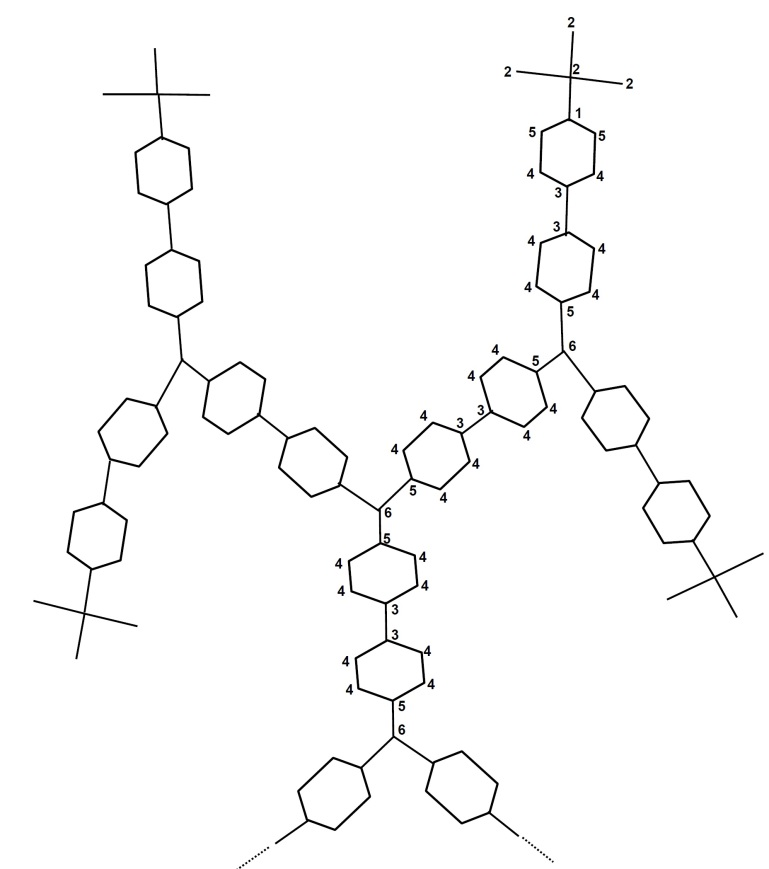
\includegraphics[width=0.7\linewidth]{img2}
\caption{The number of vertices at distance $3$ from each vertex in a third of $NSB(n)$.}
\end{figure}


\begin{table}
\label{table1}
\begin{center}
\begin{tabular}{ |c|c|c| } 
%\label{table1}
 \hline
 Type of Vertices & Num & The number of vertices at distance $3$ \\\hline 
 $1$ & $1$ & $6$ \\\hline
 $2$ & $3$ & $5$ \\\hline
 $3$ & $6$ & $4$ \\\hline
 $4$ & $6$ & $4$ \\\hline
 $5$ & $3$ & $3$ \\\hline
 $6$ & $3$ & $3$ \\\hline
 $6$ & $3$ & $3$ \\\hline 
 \vdots & \vdots & \vdots \\\hline
 $9n+7$ & $3\times 2^{n+1}$ & 4\\\hline
 $9n+8$ & $3\times 2^{n+1}$ & 5 \\\hline
 $9n+9$ & $3\times 2^{n}$ & 1\\\hline
 $9n+10$ & $3\times 2^{n}$ & 2\\\hline
 $9n+11$ & $9\times 2^{n+1}$ & 2\\\hline
 \hline
\end{tabular}
\end{center}
\caption{ Types of vertices for $NSB(n)$}
\end{table}




%%%%%%%%%%% REFERENCES %%%%%%%%%%%%%%%%
\begin{thebibliography}{99}
\bibitem{1}
R. Todeschini, V. Conosonni, {\it Hand book of Molecular Descriptors}, Weinheim: Wiley-VCH, 2000. 
\bibitem{2}
X. Li, Y. Shi, A survey on the Randic index, {\it MATCH Commun. Math. Comput.}, {\bf 59} (2008), 127-156.
\bibitem{3} 
L. Feng, W. Liu, A. Ilic, G. Yu, The degree distance of unicyclic graphs with given, {\it Graphs Comb}, {\bf 29} (2013), 449-469. 
\bibitem{4}
G. Yu, L. Feng, A. Ilic, On the eccentric distance sum of trees and unicyclic graphs, {\it J. Math. Anal. Appl}, {\bf 375} (2011), 934-944.
\bibitem{5}
G. Yu, H, Qu, L. Tang, L. Feng, On the connective eccentricity index of trees and,{\it J. Math. Anal. Appl}, {\bf 420} (2014), 1776-1786.
\bibitem{6}
L. Feng, G. Yu, K. Xu, Z. Jiang, A note on the Kirchhof index of bicyclic graphs, {\it Ars Comb}, {\bf 114} (2014), 33-40.
\bibitem{7} 
G. Yu, L. Feng, Q. Wang, Bicyclic graphs with small positive index of inertia, {\it Lin.Algebra Appl.}, {\bf 438} (2013), 2036-2045.
\bibitem{8} 
Z. Chen, M. Dehmer, Y. Shi, H. Yang, Sharp upper bounds for the Balaban index of bicyclic graphs, {\it MATCH Commun. Math. Comput. Chem}, {\bf 75} (2016), 105-128.
\bibitem{9} 
H. Wiener, "Structural determination of paran boiling points," {\it J. Am. Chem. Soc}, {\bf 69} (1947), 17-20. 
\bibitem{10}
I. Lukovits, W. Linert, Polarity{numbers of cycle containing structures}, {\it J. Chem.Inf. Comput. Sci}, {\bf 38} (1998), 715-719. 
\bibitem{11}
H. Hosoya, Y. Gao, {\it Mathematical and chemical analysis of Wiener's polarity number}, Horwood, Chichester, pp. 38-57, 2002. 
\bibitem{12} 
W. Du, X. Li, Y. Shi, Algorithms and extremal problem on Wiener polarity index, {\it MATCH Commun. Math. Comput. Chem}, {\bf 62} (2009), 235-244. 
\bibitem{13}
H. Deng, H. Xiao, F. Tang, On the extremal Wiener polarity index of trees with a given diameter, {\it MATCH Commun. Math. Comput. Chem}, {\bf 63}(2010), 257-264. 
\bibitem{14}
Hou, B. Liu, Y. Huang, The maximum Wiener polarity index of unicyclic graphs, {\it Appl. Math. Comput}, {\bf 218} (2012), 10149-10157. 
\bibitem{15}
J. Ma, Y. Shi, Z. Wang, J. Yue, On Wiener polarity index of bicyclic networks, {\it Sci.Rep}, {\bf 6} (2016), 190-211. 
\bibitem{16}
A. Behmaram, H. Yousefi Azari, A. R. Ashra, Wiener polarity index of fullerenes and hexagonal systems, {\it Appl. Math. Lett}, {\bf 25} (2012), 1510-1513.
\bibitem{17} 
Hui Lei, Tao Li, Yongtang Shi, Hua Wang, Wiener Polarity Index and Its Generalization in Trees, {\it MATCH Commun. Math. Comput. Chem}, {\bf 78} (2017), 199-212. 
\bibitem{18}
A.R. Ashrafi, M. Mirzargar, {\it Indian J. Chem.}, {\bf 47A} (2008), 538.
\bibitem{19} 
A.Karbasioun, A. R. Ashrafi, Maced, {\it J. Chem. Eng}, {\bf 28} (2009), 49. 
\bibitem{20}
M.H Khoramdel, H, Yousefi-Azari, A. R. Ashrafi, {\it Indian J. Chem.}, {\bf 47A} (2008), 1503. 
\bibitem{21}
YARAHMADI, Z., Eccentric Connectivity and Augmented Eccentric Connectivity Indices of N-Branched Phenylacetylenes Nanostar Dendrimers, {\it Iranian Journal of Mathematical Chemistry}, {\bf 1} (2010), 105-110. 
\bibitem{22}
YARAHMADI, Z. and FATH-TABAR, G.H., The Wiener, Szeged, PI, vertex PI, the first and second Zagreb indices of N-branched phenylacetylenes dendrimer, {\it MATCH Commun. Math. Comput. Chem.}, {\bf 65} (2011), no. 1, 201-208. 
\bibitem{23}
 Sara Mehdipour, Mehdi Alaeiyan, Ali Nejati, COMPUTING EDGE VERSION OF ECCENTRIC CONNECTIVITY INDEX OF NANOSTAR DENDRIMERS, {\it Kragujevac J. Sci.}, {\bf 40} (2018), 49-56.

%% example for a book
%\bibitem{gasrah} G. Gasper, M. Rahman,
%{\it Basic Hypergeometric Series}, Cambridge University Press, Cambridge (1990).


%% example for paper in journal
%\bibitem{Moak} D.S. Moak,
%The $q$-analogue of the Laguerre polynomials, {\it J. Math. Anal. Appl.}, {\bf 81} (1981), 20-47.

%% example for paper in Proc. or Collected Works
%\bibitem{rosbl} M. Rosenblum,
%Generalized Hermite polynomials and the Bose-like oscillator
%calculus, In: {\it Operator Theory: Advances and Applications},
%Birkh\"auser, Basel (1994), 369-396.

\end{thebibliography}

\end{document}
%%%%%%%%%%%%%%%%%%%%%%%%%55
